\chapter{Arhitektura i dizajn sustava}		

				
		\section{Baza podataka}
			
			\textit{Za potrebe našeg sustava koristit ćemo relacijsku bazu podataka koja svojom strukturom olakšava modeliranje znanstvene konferencije i njenih sudionika. Gradivna jedinka baze je relacija, odnosno tablica koja je definirana svojim imenom i skupom atributa. Zadaća baze podataka je brza i jednostavna pohrana, izmjena i dohvat podataka za daljnju obradu.
				Baza podataka ove aplikacije sastoji se od sljedećih entiteta:}
			
			\begin{itemize}
				\item 	\textit{Prijavljeni korisnik}
				\item 	\textit{Autor}
				\item 	\textit{Rad}
				\item 	\textit{Sekcija}
				\item 	\textit{Konferencija}
				\item 	\textit{Administrator}
				\item 	\textit{Organizator}
				\item 	\textit{Recenzent}		
			\end{itemize}
			
			\subsection{Opis tablica}
			
			
			\textbf{Prijavljeni korisnik}\space\space\space Ovaj entitet sadržava sve važne informacije o korisniku aplikacije.
				Sadrži atribute: Identifikacija, ime, prezime, adresa, naziv institucije/poduzeća, sekcija. Ovaj entitet u vezi je One-to-One s entitetom Rad preko atributa Identifikacija prijavljenog korisnika
			
			\begin{longtabu} to \textwidth {|X[6, l]|X[6, l]|X[20, l]|}
				
				\hline \multicolumn{3}{|c|}{\textbf{Prijavljeni korisnik}}	 \\[3pt] \hline
				\endfirsthead
				
				\hline \multicolumn{3}{|c|}{\textbf{Prijavljeni korisnik}}	 \\[3pt] \hline
				\endhead
				
				\hline 
				\endlastfoot
				
				\cellcolor{LightGreen} Identifikacija & INT	&  jedinstveni identifikator korisnika\\ \hline
				Ime	& VARCHAR & ime prijavljenog korisnika  	\\ \hline 
				Prezime & VARCHAR &  prezime prijavljenog korisnika \\ \hline 
				Adresa & VARCHAR	&  adresa stanovanja prijavljenog korisnika
				(ulica, kućni broj, grad, država)		\\ \hline 
				Naziv institucije poduzeća & VARCHAR	&  naziv institucije/poduzeća pod čijim pokroviteljstvom je rad proveden		\\ \hline 
				Sekcija & VARCHAR	& sekcija u koju se korisnik prijavljuje  		\\ \hline 
				Email & VARCHAR	& email adresa korisnika  		\\ \hline 
				
				
				
			\end{longtabu}
			
			
			\textbf{Autor}\space\space\space Ovaj entitet sadržava sve važne informacije o autoru nekog rada.
				Sadrži atribute: E-mail adresa, ime, prezime. Ovaj entitet u vezi je Many-to-Many s entitetom Rad
			
			
			\begin{longtabu} to \textwidth {|X[6, l]|X[6, l]|X[20, l]|}
				
				\hline \multicolumn{3}{|c|}{\textbf{Autor}}	 \\[3pt] \hline
				\endfirsthead
				
				\hline \multicolumn{3}{|c|}{\textbf{Autor}}	 \\[3pt] \hline
				\endhead
				
				\hline 
				\endlastfoot
				
				\cellcolor{LightGreen} Email adresa & VARCHAR	&  jedinstvena e-mail adresa autora\\ \hline
				Ime	& VARCHAR & ime autora  	\\ \hline 
				Prezime & VARCHAR &  prezime autora \\ \hline 
				
				
			\end{longtabu}
			
			\textbf{Rad}\space\space\space	Ovaj entitet sadržava sve važne informacije o radu predanom na konferenciju.
				Sadrži atribute: ID rada, naziv rada, identifikacija, naziv sekcije, ID konferencije. Ovaj entitet u vezi je One-to-One s entitetom Prijavljeni korisnik preko atributa Identifikacija prijavljenog korisnika, Many-to-Many s entitetom Autor te Many-to-One s entitetom Sekcija preko atributa naziv sekcije te atributa ID konferencije
			
			\begin{longtabu} to \textwidth {|X[6, l]|X[6, l]|X[20, l]|}
				
				\hline \multicolumn{3}{|c|}{\textbf{Rad}}	 \\[3pt] \hline
				\endfirsthead
				
				\hline \multicolumn{3}{|c|}{\textbf{Rad}}	 \\[3pt] \hline
				\endhead
				
				\hline 
				\endlastfoot
				
				\cellcolor{LightGreen} ID rada & INT	&  Jedinstveni identifikator rada\\ \hline
				Naziv rada	& VARCHAR & naziv rada  	\\ \hline
				Identifikacija & INT	&  jedinstveni identifikator korisnika
				(Prijavljeni korisnik.identifikacija)\\ \hline 
				\cellcolor{LightBlue} Naziv sekcije	& VARCHAR	&  naziv sekcije na koju je rad prijavljen
				(sekcija.naziv sekcije)		\\ \hline 
				\cellcolor{LightBlue} ID konferencije	& INT &  ID konferencije na čiju je sekciju rad prijavljen
				(konferencija.ID konferencije) 		\\ \hline 
				
				
				
			\end{longtabu}
			
			\textbf{Sekcija	}\space\space\space	Ovaj slabi entitet sadržava sve važne informacije o sekciji na nekoj konferenciji.
				Sadrži atribute: Naziv sekcije, ID konferencije. Ovaj entitet u vezi je Many-to-One s entitetom Konferencija preko atributa ID konferencije te u vezi One-to-Many s entitetom Rad preko atributa naziv sekcije te atributa ID konferencije
			
			\begin{longtabu} to \textwidth {|X[6, l]|X[6, l]|X[20, l]|}
				
				\hline \multicolumn{3}{|c|}{\textbf{Sekcija}}	 \\[3pt] \hline
				\endfirsthead
				
				\hline \multicolumn{3}{|c|}{\textbf{Sekcija}}	 \\[3pt] \hline
				\endhead
				
				\hline 
				\endlastfoot
				
				\cellcolor{LightGreen} Naziv sekcije & VARCHAR	&  Jedinstveni naziv sekcije 
				(jedinstven za ovu konferenciju)\\ \hline
				
				\cellcolor{LightGreen} ID konferencije	& INT &  ID konferencije na čiju je sekciju rad prijavljen
				(konferencija.ID konferencije) 		\\ \hline 
				
				
				
			\end{longtabu}
			
			\textbf{Konferencija}\space\space\space	Ovaj entitet sadržava sve važne informacije o konferenciji.
				Sadrži atribute: ID konferencije, naziv konferencije, datum održavanja. Ovaj entitet u vezi je One-to-Many s entitetom Sekcija preko atributa ID konferencije te u vezi Many-to-One s entitetom Administrator preko atributa ID administratora
			
			\begin{longtabu} to \textwidth {|X[6, l]|X[6, l]|X[20, l]|}
				
				\hline \multicolumn{3}{|c|}{\textbf{Konferencija}}	 \\[3pt] \hline
				\endfirsthead
				
				\hline \multicolumn{3}{|c|}{\textbf{Konferencija}}	 \\[3pt] \hline
				\endhead
				
				\hline 
				\endlastfoot
				
				\cellcolor{LightGreen} ID konferencije	& INT &  ID konferencije  		\\ \hline 
				
				Naziv konferencije	& VARCHAR & naziv konferencije  	\\ \hline
				
				Datum održavanja	& DATE & datum održavanja konferencije  	\\ \hline
				
				\cellcolor{LightBlue} ID administratora & INT	&  Jedinstveni ID administratora konferencije
				(administrator.ID administratora)\\ \hline
				
				
				
			\end{longtabu}
			
			\textbf{Administrator}\space\space\space	Ovaj entitet sadržava sve važne informacije o administratoru konferencije.
				Sadrži atribute: ID administratora, ime, prezime. Ovaj entitet u vezi je One-to-Many s entitetom Konferencija preko atributa ID administratora te u vezi One-to-One s entitetom Organizator preko atributa ID administratora
			
			\begin{longtabu} to \textwidth {|X[6, l]|X[6, l]|X[20, l]|}
				
				\hline \multicolumn{3}{|c|}{\textbf{Administrator}}	 \\[3pt] \hline
				\endfirsthead
				
				\hline \multicolumn{3}{|c|}{\textbf{Administrator}}	 \\[3pt] \hline
				\endhead
				
				\hline 
				\endlastfoot
				
				\cellcolor{LightGreen} ID
				administratora	& INT &  ID administratora \\ \hline 
				
				Ime	& VARCHAR & ime administratora\\ \hline
				
				Prezime	& VARCHAR & prezime administratora 	\\ \hline
				
				
			\end{longtabu}
			
			\textbf{Organizator	}\space\space\space	Ovaj entitet sadržava sve važne informacije o organizatoru konferencije.
				Sadrži atribute: ID organizatora, ime, prezime, ID administratora. Ovaj entitet u vezi je One-to-Many s entitetom Recenzent preko atributa ID organizatora te u vezi One-to-One s entitetom Administrator preko atributa ID administratora
			
			\begin{longtabu} to \textwidth {|X[6, l]|X[6, l]|X[20, l]|}
				
				\hline \multicolumn{3}{|c|}{\textbf{Organizator}}	 \\[3pt] \hline
				\endfirsthead
				
				\hline \multicolumn{3}{|c|}{\textbf{Organizator}}	 \\[3pt] \hline
				\endhead
				
				\hline 
				\endlastfoot
				
				\cellcolor{LightGreen} ID
				organizatora & INT &  ID organizatora\\ \hline 
				
				Ime	& VARCHAR & ime organizatora\\ \hline
				
				Prezime	& VARCHAR & prezime organizatora 	\\ \hline
				
				\cellcolor{LightBlue} ID
				administratora	& INT &  ID administratora
				(administrator.ID administratora) \\ \hline 
				
				
			\end{longtabu}
			
			\textbf{Recenzent}\space\space\space	Ovaj entitet sadržava sve važne informacije o recenzentu.
				Sadrži atribute: ID recenzenta, ime, prezime, ID organizatora. Ovaj entitet u vezi je Many-to-Many s entitetom Rad te u vezi Many-to-One s entitetom Organizator preko atributa ID organizatora
			
			\begin{longtabu} to \textwidth {|X[6, l]|X[6, l]|X[20, l]|}
				
				\hline \multicolumn{3}{|c|}{\textbf{Recenzent}}	 \\[3pt] \hline
				\endfirsthead
				
				\hline \multicolumn{3}{|c|}{\textbf{Recenzent}}	 \\[3pt] \hline
				\endhead
				
				\hline 
				\endlastfoot
				
				\cellcolor{LightGreen} ID
				recenzenta & INT &  ID recenzenta\\ \hline 
				
				Ime	& VARCHAR & ime recenzenta\\ \hline
				
				Prezime	& VARCHAR & prezime recenzenta 	\\ \hline
				
				\cellcolor{LightBlue} ID
				organizatora	& INT &  ID organizatora
				(organizator.ID organizatora) \\ \hline 
				
				
			\end{longtabu}
			
			
			\subsection{Dijagram baze podataka}
			
			\begin{figure}[H]
				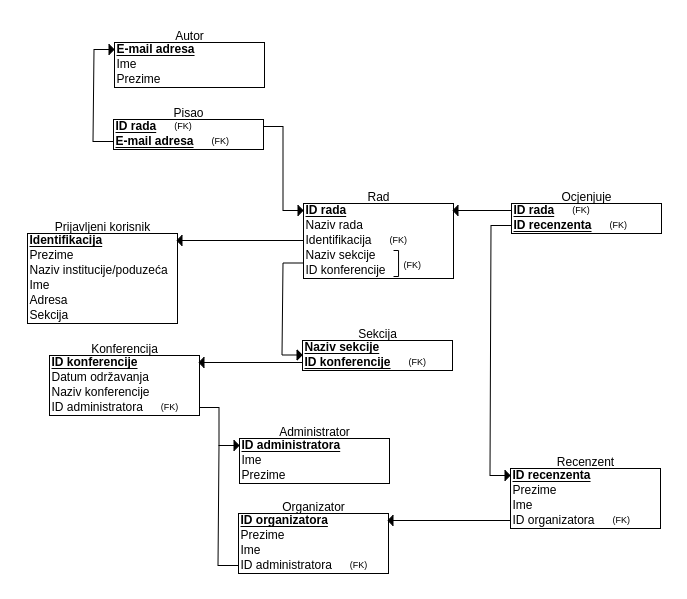
\includegraphics[width=.9\linewidth]{slike/ERdijagram.png} %veličina u odnosu na širinu linije
				\centering
				\caption{Relacijska shema baze podataka}
				\label{fig:RelShema} %label mora biti drugaciji za svaku sliku
			\end{figure}
			
			\eject
			
			
			
			
			
		\section{Dijagram razreda}
		
			\noindent \underbar{\textbf{Opis dijagrama razreda:}}
			\begin{packed_item}
				\item \textbf{Konferencija} Središnji razred koji predstavlja konferenciju
				\item \textbf{Administrator} Predstavlja administratora sustava, ima na raspolaganju sljedeći skup funkcionalnosti sustava:
				\begin{packed_item}
					\item Stvaranje nove konferencije
					\item Pregled statističkih podataka o korisnicima
					\item Izmjenu podataka registriranih korisnika
					\item Određivanje organizatora konferencije
				\end{packed_item}
				\item \textbf{Sekcija}  Konkretna sekcija na nekoj od konferencija
				\item \textbf{Recenzent} Predstavlja recenzenta na konferenciji, može pregledavati, \linebreak ocjenjivati i preuzimati radove na svoje računalo
				\item \textbf{Sudionik konferencije} Predstavlja sudionika na konferenciji,  omogućavaju \linebreak mu se sljedeće akcije:
				\begin{packed_item}
					\item Prijava na konferenciju
					\item Izmjena vlastitih podataka te promjena lozinke
					\item Učitavanje rada u pdf formatu
				\end{packed_item}
				\item \textbf{Adresa sudionika} Predstavlja adresu određenog sudionika
				\item \textbf{Organizator konferencije} Predstavlja organizatora konferencije,  omogućavaju \linebreak mu se sljedeće akcije:
				\begin{packed_item}
					\item Pregled i potvrda prijava recenzenata za određenu konferenciju
					\item Slanje poruka putem elektroničke pošte svim sudionicima
					\item Pregled i izmjena podataka sudionika konferencije
					\item Preuzimanje radova sudionika konferencije
				\end{packed_item}
				\item \textbf{Znanstveni rad} Predstavlja znanstveni rad sudionika na konferenciji
				\item \textbf{Ocjena} Predstavlja jednu od  tri ocjene recenzenta u enumeraciji:
				\begin{packed_item}
					\item Prihvati rad
					\item Prihvati rad uz doradu
					\item Odbij rad
				\end{packed_item}
			\end{packed_item}
			
			\begin{figure}[H]
				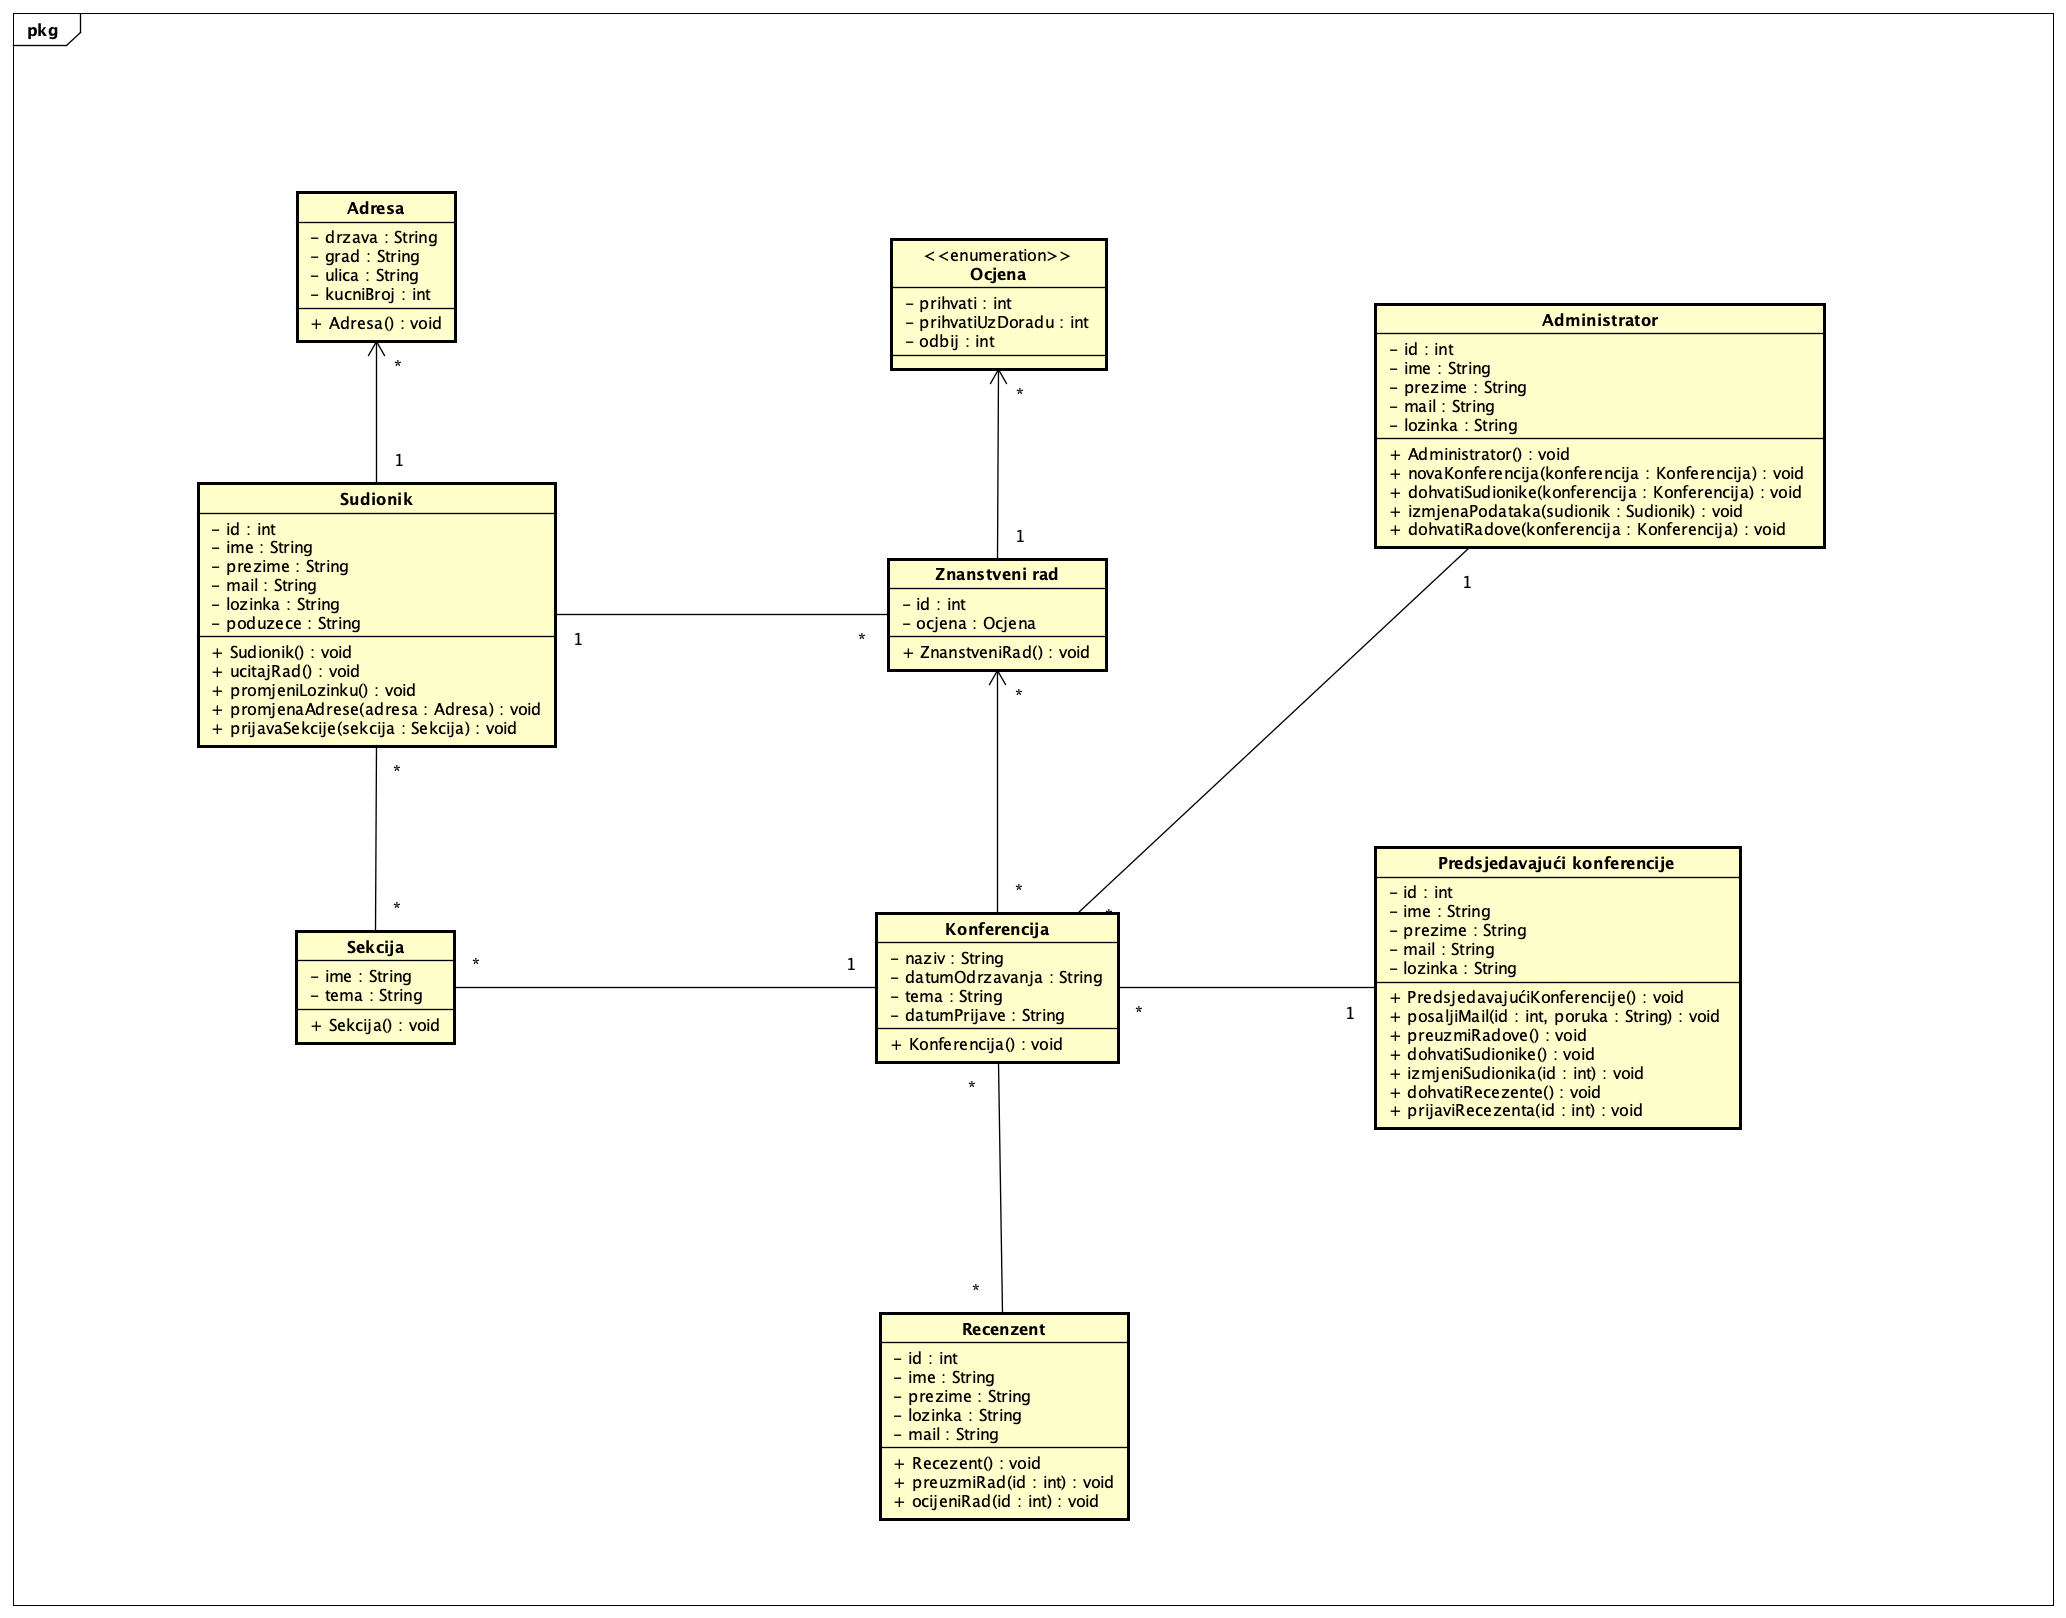
\includegraphics[width=1\linewidth]{slike/ClassDiagramSlika} %veličina u odnosu na širinu linije
				\centering
				\caption{Dijagram razreda}
				\label{Class Diagram} %label mora biti drugaciji za svaku sliku
			\end{figure}
		
			\eject
			
		\section{Dijagram stanja}
			Dijagram stanja prikazuje stanje objekta te prijelaze iz jednog stanja u drugo temeljene na događajima. Na slici 4.3 prikazan je dijagram stanja za Korisnika. Nakon uspješne prijave korisniku se prikazuje početna stranica na kojoj može odabrati više opcija. Klikom na Popis konferencija mu se prikazuju konferencije na koje se dalje može prijaviti, a u prijavi odabrati sekciju, unijeti podatke i naposlijetku potvrditi prijavu. Klikom na Učitavanje rada, uz uvjet da mu je odobrena prijava u sekciju te da nije isteklo vrijeme za učitavanje rada, može učitati rad te ga onda poslati. Klikom na Postavke, korisnik može urediti vlastite podatke pa onda izmijenjene podatke spremiti. Također, korisnik u Postavkama može i izbrisati svoj korisnički račun. Klikom na Moji radovi, korisnik može pogledati informacije o svojim radovima, može dohvatiti i urediti učitani rad te onda pohraniti promjene. Korisnik također može klikom na Prijava za recenziranje ispuniti obrazac prijave za recenziranje te ispunjeni obrazac potvrditi i poslati na odobrenje.
			
			\begin{figure}[H]
				\includegraphics[width=1\linewidth]{slike/"Dijagram stanja"} %veličina u odnosu na širinu linije
				\centering
				\caption{Dijagram stanja}
				\label{State Diagram - Korisnik} %label mora biti drugaciji za svaku sliku
			\end{figure}
			
			\eject
		
		\section{Dijagram aktivnosti}
			Dijagram aktivnosti primjenjuje se za opis modela toka upravljanja ili toka podataka. Ne upotrebljava se za modeliranje događajima poticanog ponašanja. U modeliranju toka upravljanja svaki novi korak poduzima se nakon završenog prethodnog, a naglasak je na jednostavnosti. Na dijagramu 4.4 prikazan je proces prijave za sudjelovanje na konferenciji. Korisnik unese podatke za prijavu u sustav, odabere popis konferencija te odabere konferenciju i sekciju u njoj. Naposljetku, korisnik unese podatke za prijavu te ga aplikacija vrati na početnu stranicu.
			
			\begin{figure}[H]
				\includegraphics[width=1\linewidth]{slike/"Dijagram aktivnosti"} %veličina u odnosu na širinu linije
				\centering
				\caption{Dijagram aktivnosti}
				\label{Activity Diagram - Prijava za sudjelovanje na konferenciji} %label mora biti drugaciji za svaku sliku
			\end{figure}
			
			\eject
			
		\section{Dijagram komponenti}
			Dijagram komponenti na slici 4.5 opisuje organizaciju i međuovisnost komponenti, interne strukture i odnose prema okolini. Preko sučelja za dohvat datoteka i JSON-a pristupa se app.js komponenti. Frontend se sastoji od HTML datoteka koje se nalaze u direktoriju "views", dok je Javascript kod backenda koji je zadužen za upravljanje rutama u diretkriju "routes".
			Postgres je zadužen za dohvaćanje tablica iz baze podataka pomoću SQL upita. Podaci koji su pristigli dalje se šalju u queries.js.
			
			\begin{figure}[H]
				\includegraphics[width=1\linewidth]{slike/"Dijagram komponenti"} %veličina u odnosu na širinu linije
				\centering
				\caption{Dijagram komponenti}
				\label{Component Diagram} %label mora biti drugaciji za svaku sliku
			\end{figure}		